\chapter{Business use cases}
\label{business-uc}

\par The business use case diagram is in figure
\ref{fig:business-use-case-diagram}. Note that there are no interested
stakeholders displayed in the diagram. This was done for the sake of
simplicity because displaying them would cause a lot of crossings. They are of
course included in the corresponding section in each use case.

\begin{figure}[H]
	\begin{centering}
		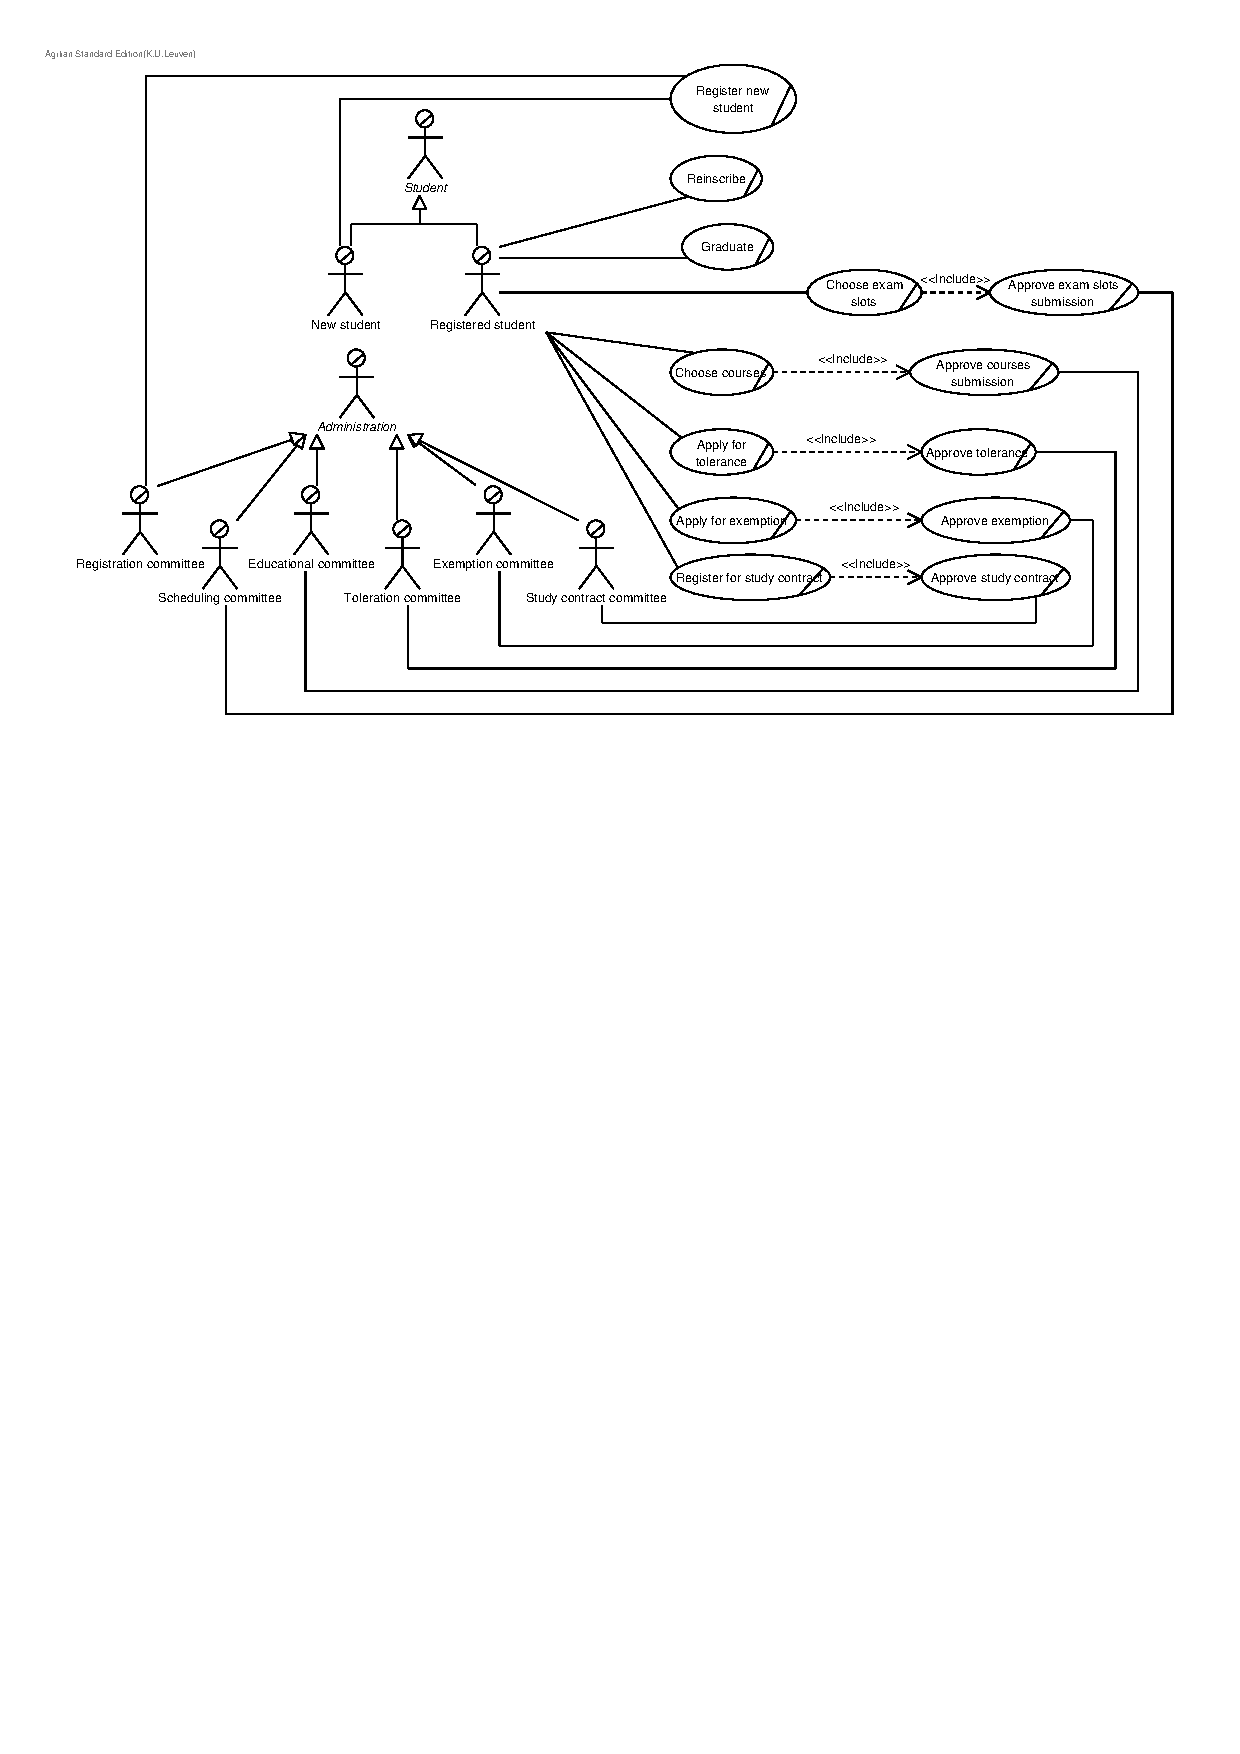
\includegraphics[width=\paperwidth,
		angle=90]{figs/business-use-case-diagram.pdf}
		\caption{Business use case diagram}
		\label{fig:business-use-case-diagram}
	\end{centering}
\end{figure}

\section{Register new student}
\label{register-new-student}

\begin{description}
	\item[Business Event Description] \
	\par A student wants to register at the Wellington
	University
	\item[Business Use Case Name] \
	\par Register new student
	\item[Triggering business event] \
	\par A student wants to register at the Wellington
	University. He is completely new and hasn't studied at Wellington before. He
	goes to the student administration building of Wellington University to make
	his inscription.
	\item[Preconditions] \ 
	\begin{itemize}
		\item Student hasn't yet studied at Wellington University.
		\item Student has a high school degree.
	\end{itemize}
	\item[Active stakeholders] \ 
	\begin{itemize}
	  	\item Student: wants to study at Wellington University.
		\item Registration employee: needs to complete the inscription of the student.
	\end{itemize}
	\item[Interested stakeholders] \ 
		\begin{itemize}
		  \item Board of the university: interested in new students.
		\end{itemize}
	\item[Normal business flow] \
	\begin{enumerate}
	  	% 1
	  	\item The student goes to the student administration building of Wellington
	  	University.
	  	% 2
	  	\item The student hands over the required information at the registration
	  	desk: home address, residence address, phone numbers, birth date, passport
	  	picture, register number, diplomas, if necessary evidence of matriculation.
	  	% 3
	  	\item The registration employee checks if the provided information is enough
	  	and is correct.
	  	% 4
	  	\item The registration employee makes the right documents: invoice,
	  	inscription attest.
	  	% 5
	  	\item The registration employee prints the student card with a unique
	  	student number and the passport picture of the student on it.
	  	% 6
	  	\item The registration employee grabs a few other documents like some
	  	folders and a free buss card.
	  	% 7
	  	\item The registration employee hands all these documents and student card
	  	over to the student.
	  	% 8
	  	\item The student accepts all these documents and is now successfully
	  	inscribed to Wellington University.
	\end{enumerate}
	\item[Alternative business flow] \ 
	\begin{description}
  		\item[3a] The registration employee notices that some documents are missing
  		because the student has forgotten to bring them.
  		\begin{enumerate}
  			\item The registration employee makes the student aware that he/she
  			can't be inscribed without these documents.
  			\item The student leaves to retrieve the missing documents.
  			\item The student returns at the student administration to restart his/her
  			inscription.
  			\item Go to normal flow 4.
		\end{enumerate}
	\end{description}
	\item[Exception business flow] \
	\begin{description}
		\item[3a] after having checked the information provided by the student, the
		registration employee notices that some documents are missing. This time not
		because the student has forgotten them, but because the student just doesn't
		have these documents (high school diploma, evidence of having passed a
		matriculation, \ldots).
		\begin{enumerate}
		  \item The registration employee makes the student aware that he/she can't be
		  inscribed without these documents.
		  \item The student leaves and can't be inscribed until he obtains the missing
		  documents.
		\end{enumerate}
	\end{description}
	\item[Outcome (postcondition)] \
	\par The student is now fully inscribed at Wellington University and has
	received all the according documents, folders, buss card and student card.
\end{description}

\section{Register for study contract}

\begin{description}
	\item[Business Event Description] \ 
		\par The student wants to register for a diploma contract.
	\item[Business Use Case Name] \ 
		\par Register for study contract
	\item[Triggering business event] \ 
		\par The student wants to register for a diploma contract and decides to take the necessary steps.
	\item[Preconditions] \ 
	\begin{itemize}
		\item The student has to be a registered student at Wellington University and
		hence has a student card.
	\end{itemize}
	\item[Active stakeholders] \ 
	\begin{itemize}
		\item Student: wants to be registered for a diploma contract.
		\item Study contract committee: controls the approval or disapproval of the
		contract the student wishes to obtain.
	\end{itemize}
	\item[Interested stakeholders] \ 
		\begin{itemize}
		\item University board: interested in new students, contract determines the
		inscription fee.
		\item Faculties: interested in new students that follow a study contract supervised
		by them
		\end{itemize}
	\item[Normal business flow] \ 
	\begin{enumerate}
	  	% 1
	  	\item The student takes the form for starting a new study contract.
	  	% 2
	  	\item The student fills in the required identification information by using
	  	his student card (with on it his unique student number).
	  	% 3
	  	\item The student chooses to register for a diploma contract.
	  	% 4
	  	\item The student chooses the bachelor or master contract of his choice.
	  	% 5
	  	\item The student sends the form to the study contract committee.
	  	% 6
	  	\item The study contract committee receives and approves the form,
	  	\textbf{include} \emph{(UC3: Approve study contract)}.
	\end{enumerate}
	\item[Alternative business flow] \ 
	\begin{description}
		\item[3a] instead of a diploma contract the student chooses to register for a
		credit contract. 
		\begin{enumerate}
		  \item Resume at step 5 of the basic flow.
		\end{enumerate}
		\item[3b] instead of a diploma contract the student chooses to register for an
		exam contract. 
		\begin{enumerate}
		  \item Resume at step 5 of the basic flow.
		\end{enumerate}
	\end{description}
	\item[Exception business flow] \ 
	\begin{description}
		\item[6a] If the check of the study contract committee comes out negative
		(e.g. he wants to follow a master study while he still has to follow a
		full bachelor year), then The student can't follow the chosen diploma contract.
		\begin{enumerate}		
		  \item The study contract committee sends a disapproval message to the
		  student.
		  \item The student receives the disapproval message, and is not allowed to
		  follow the chosen diploma contract.
		  \item The student can try to register for another diploma contract by
		  returning to step 1 in the normal flow.
		\end{enumerate}
	\end{description}
	\item[Outcome (postcondition)] \
		\par The student now follows the chosen study contract. The faculty who
		supervises that contract is aware that a new student has signed up.
\end{description}

\section{Approve study contract}

\begin{description}
	\item[Business Event Description] \ 
		\par After a student has registered for a study contract, this contract needs an
		approval to see if it doesn't violate any admission requirements.
	\item[Business Use Case Name] \ 
		\par Approve study contract
	\item[Triggering business event] \ 
		\par Whenever a student sends a study contract, this will trigger the
		approval procedure.
	\item[Preconditions] \
	\begin{itemize}
		\item The study contract committee has received the registration form.
	\end{itemize}
	\item[Active stakeholders] \ 
	\begin{itemize}
		\item Study contract committee: checks the registration form and approves it.
	\end{itemize}
	\item[Interested stakeholders] \ 
		\begin{itemize}
		\item Faculties: interested in new students that follow a study contract supervised
		by them
		\item Student: wants that his study contract application is approved
		\end{itemize}
	\item[Normal business flow] \ 
	\begin{enumerate}
	  	% 1
	  	\item The study contract committee glances through the form. 
	  	% 2
	  	\item The study contract committee verifies that the registration is a valid
	  	one.
	  	% 3
	  	\item The study contract committee approves the registration.
	  	% 4
	  	\item The study contract committee sends an approval message to the
	  	student.
	  	% 5
	  	\item The student receives the approval message and is now allowed to follow
	  	the diploma contract.
	\end{enumerate}
	\item[Alternative business flow] \
		\par None
	\item[Exception business flow] \ 
	\begin{description}
		\item[2a] If the student's submitted program is a credit or exam contract and
		the student has already registered for another contract of that same type
		within the same faculty, then the registration is rejected.
		\begin{enumerate}
		  	\item The study contract committee sends a disapproval message to the
		  	student.
		  	\item The student receives the disapproval message, and is not allowed to
		  	follow the chosen diploma contract.
		  	\item The student can try to register for another contract.
		\end{enumerate}
		\item[2b] If the student's submitted program is about a phase X where the
		student did not yet complete phase X-1, then the registration is rejected.
		\begin{enumerate}
		  	\item The study contract committee sends a disapproval message to the
		  	student.
		  	\item The student receives the disapproval message, and is not allowed to
		  	follow the chosen diploma contract.
		  	\item The student can try to register for another contract.
		\end{enumerate}
		\item[2c] If the student's submitted program is about a master where the
		student did not yet complete the preceding bachelor, the registration is
		rejected.
		\begin{enumerate}
		  	\item The study contract committee sends a disapproval message to the
		  	student.
		  	\item The student receives the disapproval message, and is not allowed to
		  	follow the chosen diploma contract.
		  	\item The student can try to register for another contract.
		\end{enumerate}
	\end{description}
	\item[Outcome (postcondition)] \ 
		\par The student's study contract is approved and he can continue to choose
		courses for this contract.
\end{description}


\section{Choose courses}

\begin{description}
	\item[Business Event Description] \ 
		\par The student decides it's time to choose his courses that are part of his
		contract(s). At the beginning of a study year the student chooses his courses
		for the whole year, at the beginning of the second semester the student can
		choose (and hence change) his courses for the second semester.
	\item[Business Use Case Name] \ 
		\par Choose courses
	\item[Triggering business event] \ 
		\par The student decides it's time to choose his courses that are part of his
		contract(s) and takes the necessary steps.
	\item[Preconditions] \
	\begin{itemize}
		\item The student is registered for at least 1 study contract.
	\end{itemize}
	\item[Active stakeholders] \ 
	\begin{itemize}
		\item Student: wants to choose his courses for the year or second semester.
		\item Educational Committee: supervises that the courses selected by the
		student are allowed to be taken by the student.
	\end{itemize}
	\item[Interested stakeholders] \ 
	\begin{itemize}
		\item Didactical team of the courses the student wants to follow.
	\end{itemize}
	\item[Normal business flow] \
	\begin{enumerate}
	  	% 1
	  	\item The student takes the form for choosing his courses.
	  	% 2
	  	\item The student provides the necessary identifying information (found on
	  	his student card). 
	  	% 3
	  	\item The student assigns for which study contract (for which he is
	  	registered) he wants to choose his courses.
	  	% 4
	  	\item The student chooses the courses.
	  	% 5
	  	\item The student sends the form to the educational committee.
	  	% 6
	  	\item The educational committee receives and checks the courses
	  	configuration and approves the configuration, \textbf{include} \emph{(UC5:
	  	Approve courses submission)}.
	\end{enumerate}
	\item[Alternative business flow] \
	\begin{description}
		\item[4a]If the student has more than 1 study contract he has to
		repeat the steps 1 - 4 of the basic flow for each study contract.
			\begin{enumerate} 
	  			\item The student sends all forms to the educational committee.
			\end{enumerate}
	\end{description}
	\item[Exception business flow] \ 
	\begin{description}
		\item[6a] If the educational committee doesn't approve
		the chosen courses (e.g. because of entry requirements) then,
		\begin{enumerate}
		 	\item The educational committee sends a disapproval message to the student.
		 	\item The student receives the disapproval message and is not allowed to
		 	follow the chosen courses.
		 	\item Return to step 4 of the normal flow.
		\end{enumerate}
	\end{description}
	\item[Outcome (postcondition)] \  
		\par The student is allowed to follow the chosen courses of his registered
		study contracts.
\end{description}

\section{Approve courses submission}
\begin{description}
	\item[Business Event Description] \ 
		\par The educational committee receives an application for chosen courses from
		a student and needs to check if the student can really take these courses.
	\item[Business Use Case Name] \ 
		\par Approve Courses Submission
	\item[Triggering business event] \ 
		\par The educational committee receives an application for chosen courses.
	\item[Preconditions] \
	\begin{itemize}
		\item The educational committee has received the prefered selection of courses
		from the student.
	\end{itemize}
	\item[Active stakeholders] \ 
	\begin{itemize}
		\item Educational committee: checks if the selection of chosen courses
		received from the student is valid.
	\end{itemize}
	\item[Interested stakeholders] \ 
		\begin{itemize}
		\item University board: interested in new students, contract determines the
		inscription fee.
		\item Student: wants to see his chosen courses selection approved.
		\end{itemize}
	\item[Normal business flow] \ 
	\begin{enumerate}
	  	% 1
	  	\item The educational committee sees that the study contract of the student
	  	is a diploma contract.
	  	% 2
	  	\item The educational committee checks that if the student is a first year
	  	student he has chosen all the courses of the first phase of that program or
	  	that he has possible exemptions (e.g. from another education at the
	  	Wellington university or another university.)
	  	% 3
	  	\item The educational committee checks that the student meets all the entry
	  	requirements for the chosen courses.
	  	% 4
	  	\item The educational committee checks that if the student is a full-time
	  	student, the total number of taken study points ranges from 40 to 75. 
	  	% 5
	  	\item The educational committee concludes all the checks come out positive.
	\end{enumerate}
	\item[Alternative business flow] \
		\begin{description}
		\item[1a] The educational committee sees that the study contract of the
		student is a credit contract. 
			\begin{enumerate}
			  \item Resume the normal flow at step 3.
			\end{enumerate}
		\item[1b] The educational committee sees that the study contract of the
		student is an exam contract. 
			\begin{enumerate}
			  \item Resume the normal flow at step 3.
			\end{enumerate}
		\item[1c] The educational committee sees that the study contract of the
		student is a combination of various study contracts.
			\begin{enumerate}
			  \item The educational committee checks that the student doesn't try to
			  follow several credit contracts or exam contracts for courses under the
			  supervision of the same faculty.
			  \item The educational committee checks that the student didn't chose
			  an unfinished course that is included in different contracts at the same
			  time.
			  \item Resume the basic flow at step 3.
			\end{enumerate}
		\end{description}
		\item[4c] In case the student is a part-time student, the committee checkts
		that the total number of study points ranges from 0 to 30.
	\item[Exception business flow] \ 
	\begin{description}
		\item[5a] if one or more of the checks comes out negative then,
		\begin{enumerate}
		  \item The student is notified of the rejection of his selection.
		\end{enumerate}
	\end{description}
	\item[Outcome (postcondition)] \ 
		\par The selection of chosen courses is approved.
\end{description}

\section{Apply for exemption}

\begin{description}
	\item[Business Event Description] \ 
		\par The student intends to register for at least one study program in the
		upcoming acadmic year. In one of those programs, there is a course he/she
		thinks he/she can substitute it with a course he/she followed in another
		program. This course is not necessarily taught at the university of
		Wellington.
	\item[Business Use Case Name] \ 
		\par Apply for exemption
	\item[Triggering business event] \ 
		\par The student thinks he can acquire an exemption for a course of a
		studyprogram he intends to follow.
	\item[Preconditions] \
	\begin{itemize}
		\item The student is registrered at the university of the Wellington.
		\item The student wants to follow at least one study program during the
		upcoming academic year. 
		\item The student has followed at least one course in a previous academic year
		(which can act as a substitute).
	\end{itemize}
	\item[Active stakeholders] \ 
	\begin{itemize}
		\item Student
	\end{itemize}
	\item[Interested stakeholders] \ 
		\begin{itemize}
		\item Exemption committee
		\end{itemize}
	\item[Normal business flow] \ 
	\begin{enumerate}
	  	% 1
	  	\item The student takes the form to acquire an exemption.
	  	% 2
	  	\item The student fills in his identification information, i.e. the unique
	  	student number on his student card.
	  	% 3
	  	\item The student fills in the course that he/she wants to acquire the
	  	exemption for. 
	  	% 4
	  	\item The student fills in the course that he/she thinks can act as a
	  	substitute for the course in the previous bullet. He/she also provides the
	  	institute where that course was taught.
	  	% 5
	  	\item The student also fills in the study program to which the exemption
	  	applies.
	  	% 6
	  	\item A motivation why he/she justifies the exemption (e.g. a comparison of
	  	the similarity of the contents of both courses).
	  	% 7
	  	\item The student sends the form to the exemption committee of the faculty
	  	which supervises the studyprogram, \textbf{include} \emph{(UC7: Approve
	  	exemption)}.
	\end{enumerate}
	\item[Alternative business flow] \ 
		\par None
	\item[Exception business flow] \
		\par None
	\item[Outcome (postcondition)] \ 
		\par The student's exemption is approved.
\end{description}
\section{Approve exemption}

\begin{description}
	\item[Business Event Description] \ 
		\par The exemption committee has received an application for an exemption
		from a student and needs to check if the exemption can be granted.
	\item[Business Use Case Name] \ 
		\par Approve exemption
	\item[Triggering business event] \ 
		\par The exemption committee has received application for an exemption from a
		student.
	\item[Preconditions] \
	\begin{itemize}
		\item The exemption committee has received application for an exemption from a
		student.
	\end{itemize}
	\item[Active stakeholders] \ 
	\begin{itemize}
		\item Exemption committee: checks that the exemption can be granted.
	\end{itemize}
	\item[Interested stakeholders] \ 
		\begin{itemize}
		\item Student: wants to know if his exemption is granted.
		\item Educational Committee: can incorporate any tolerances in approving
		study contracts.
		\end{itemize}
	\item[Normal business flow] \ 
	\begin{enumerate}
	  	% 1
	  	\item The exemption committee reads through the form. 
	  	% 2
	  	\item The exemption committee checks that the specific course is indeed a
	  	valid substitute (e.g. equal amount of work, similar topics, \ldots)
	  	% 3
	  	\item The exemption committee approves the exemption.
	  	% 4
	  	\item The exemption committee notifies the student of the approval.
	  	% 5
	  	\item The student is notified.
	\end{enumerate}
	\item[Alternative business flow] \ 
		\par None
	\item[Exception business flow] \ 
	\begin{description}
		\item[6a]  If the exemption committee rejects the exemption then,
		\begin{enumerate}
		  \item The exemption committee sends a disapproval message to the student.
		  \item The student receives the disapproval message.
		\end{enumerate}
	\end{description}
	\item[Outcome (postcondition)] \ 
		\par The student is granted the chosen exemption.
\end{description}

\section{Apply for tolerance}

\begin{description}
	\item[Business Event Description] \ 
		\par After the deliberation of the last exam period (August - September) the
		student decides to tolerate a certain course. %TODO kan toch ook na Juni, mss
		% Kerst ?
	\item[Business Use Case Name] \ 
		\par Apply for tolerance
	\item[Triggering business event] \ 
		\par The student didn't pass for a certain course, even after the last
		examination period (August - September), and decides to tolerate it.
	\item[Preconditions] \
	\begin{itemize}
		\item The student obtained a score of 8 or 9 as highest score on an
		examination of a certain course (which he wants to tolerate), even after the
		last examination period (August - September).
	\end{itemize}
	\item[Active stakeholders] \ 
	\begin{itemize}
		\item Student: wants to obtain a tolerance for a certain course.
	\end{itemize}
	\item[Interested stakeholders] \ 
		\begin{itemize}
		\item Tolerance committee: checks if the student can indeed tolerate the
		course and will be notified when the student sends the form.
		\end{itemize}
	\item[Normal business flow] \ 
	\begin{enumerate}
	  	% 1
	  	\item The student takes the form for tolerating a course.
	  	% 2
	  	\item The student provides the necessary identifying information (found on
	  	his student card).
	  	% 3
	  	\item The student assigns for which course he wants to ask for a toleration.
	  	% 4
	  	\item The student sends the form to the tolerance committee.
	  	% 5
	  	\item The tolerance committee receives and checks the form and approves the
	  	tolerance, \textbf{include} \emph{(UC9: Approve tolerance)}.
	\end{enumerate}
	\item[Alternative business flow] \ 
		\par None
	\item[Exception business flow] \ 
		\par None
	\item[Outcome (postcondition)] \ 
		\par The student has completed the course he wanted to tolerate but he lost
		the study points of the tolerated course.
\end{description}

\section{Approve tolerance}

\begin{description}
	\item[Business Event Description] \ 
		\par Not every student passes for every single course. Students can, however,
		tolerate shortcomings under certain restrictions. Every toleration request
		needs to be (dis)approved which is performed by the toleration committee.
	\item[Business Use Case Name] \ 
		\par Approve tolerance
	\item[Triggering business event] \ 
		\par The toleration committee has received a request for a toleration of a
		certain course from a certain student. The committee, however, has to check that the
		request can be granted. 
	\item[Preconditions] \
	\begin{itemize}
		\item The toleration committee has received the tolerance form.
	\end{itemize}
	\item[Active stakeholders] \ 
	\begin{itemize}
		\item Toleration committee: checks to see if the tolerance can be granted
	\end{itemize}
	\item[Interested stakeholders] \ 
		\begin{itemize}
		\item Student: wants to know if his request is accepted
		\item Educational committee: can incorporate any tolerances in approving study
		contracts.
		\end{itemize}
	\item[Normal business flow] \ 
	\begin{enumerate}
	  	% 1
	  	\item The toleration committee glances through the form. 
	  	% 2
	  	\item The toleration committee checks that the student has enough tolerance
	  	budget for the toleration.
	  	% 3
	  	\item The toleration committee tolerates the shortcoming.
	  	% 6
	  	\item The tolerance committee sends an approval message to the student and
	  	notifies the educational committee of this tolerance.
	  	% 7
	  	\item The student receives the approval message and is now granted a
	  	tolerance for the chosen course.
	\end{enumerate}
	\item[Alternative business flow] \ 
		\par None
	\item[Exception business flow] \ 
	\begin{description}
		\item[2a] If the tolerance committee comes out negative (e.g. because of a
		lack of tolerance budget) then,
		\begin{enumerate}
		  \item The tolerance committee sends a disapproval message to the student.
		  \item The student receives the disapproval message and is not granted the
		  chosen tolerance.
		\end{enumerate}
	\end{description}
	\item[Outcome (postcondition)] \ 
		\par The tolerance application of the student is approved.
\end{description}

\section{Choose exam slots}

\begin{description}
	\item[Business Event Description] \ 
		\par After choosing his preferred courses, the student decides to choose an
		exam slot for each of these courses.
	\item[Business Use Case Name] \ 
		\par Choose exam slots
	\item[Triggering business event] \ 
		\par The student wants to choose his exam slots for his preferred courses.
	\item[Preconditions] \
	\begin{itemize}
		\item The student has made the selection of the courses he wants to take.
	\end{itemize}
	\item[Active stakeholders] \ 
	\begin{itemize}
		\item Student: wants to choose when he does each exam
	\end{itemize}
	\item[Interested stakeholders] \ 
		\begin{itemize}
		\item Lector(s): wants to know when he has to interrogate which student about
		the courses he teaches.
		\end{itemize}
	\item[Normal business flow] \ 
	\begin{enumerate}
	  	% 1
	  	\item The student takes the form for choosing exam slots.
	  	% 2
	  	\item The student provides the necessary identifying information (found on
	  	his student card).
	  	% 3
	  	\item The student chooses an exam slot for each course.
	  	% 4
	  	\item The student sends the form to the scheduling committee.
	  	% 5
	  	\item The scheduling committee checks the form and approves the chosen exam
	  	slots, \textbf{include} \emph{(UC11: Approve Exam Slots Submission)}.
	\end{enumerate}
	\item[Alternative business flow] \
		\par None 
	\item[Exception business flow] \ 
		\par None
	\item[Outcome (postcondition)] \ 
		\par The chosen exam slots are approved by the scheduling committee and the
		student is notified of this fact.
\end{description}
\section{Approve exam slots submission}

\begin{description}
	\item[Business Event Description] \ 
		\par The scheduling committee received a message (i.e. submission) containing
		the preferred exam slots of a student and now needs to check of this
		configuration of exam slots is allowed.
	\item[Business Use Case Name] \ 
		\par Approve exam slots submission
	\item[Triggering business event] \ 
		\par The scheduling committee receives a submission of the preferred exam
		slots of a student.
	\item[Preconditions] \
	\begin{itemize}
		\item The scheduling committee has received the submission of the preferred
		exam slots of a student.
	\end{itemize}
	\item[Active stakeholders] \ 
	\begin{itemize}
		\item Scheduling committee: checks the preferred exam slots submission of the
		student.
	\end{itemize}
	\item[Interested stakeholders] \ 
		\begin{itemize}
		\item Student: wants that his preferred exam slots submission is approved.
		\end{itemize}
	\item[Normal business flow] \ 
	\begin{enumerate}
	  	% 1
	  	\item The scheduling committee checks that no chosen slots overlap.
	  	% 2
	  	\item The scheduling committee checks that no chosen slots are overbooked.
	  	% 3
	  	\item The scheduling committee notices that all checks succeed.
	  	% 4
	  	\item The scheduling committee sends an approval message to the student.
	  	% 5
	  	\item The student receives the approval message and is now allowed to take
	  	the exams on the chosen slots.
	\end{enumerate}
	\item[Alternative business flow] \ 
		\par None
	\item[Exception business flow] \ 
	\begin{description}
		\item[3a] if the scheduling committee notices that some checks have failed
		then, 
		\begin{enumerate}
		  \item The scheduling committee sends a disapproval message to the student.
		  \item The student receives the disapproval message and has to change his
		  chosen exam slots to a valid configuration.
		\end{enumerate}
	\end{description}
	\item[Outcome (postcondition)] \ 
		\par The student is allowed to take his exams on the chosen exam slots and is
		notified of this fact by the scheduling committee.
\end{description}

